\section{Introduction}
\label{introduction}

% state the learning objective 
The aim of this laboratory work regarding the topics studied in the first three weeks of the course was to analyse a circuit constituted by an independent voltage source, an independent current source, a voltage controlled dependent current source, a current controlled dependent voltage source and seven resistors, as shown in the Figure 1 below.
 For this, a theorical analysis was made using both node and mesh methods, whose results will be discussed in Section 2. To validate these results, a simulation was conducted, as will appear in Section 3.


The results were then compared and the conclusions of the group summarized in Section 4.


\begin{figure}[ht] \centering
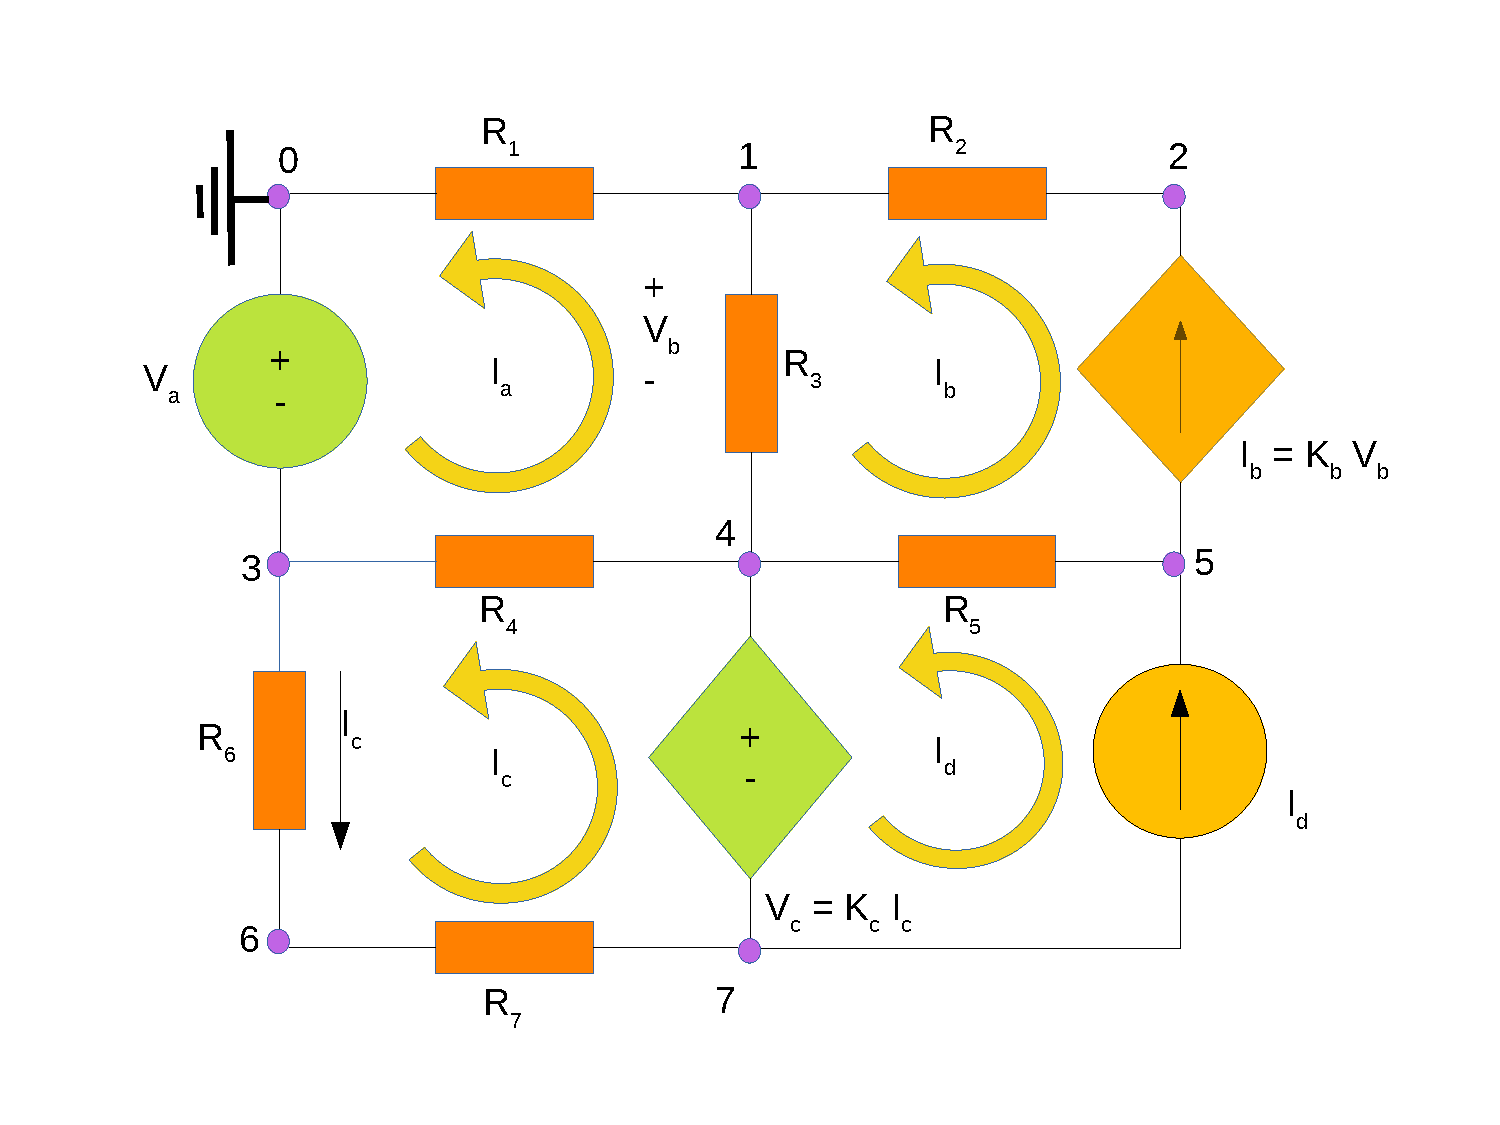
\includegraphics[width=0.9\linewidth]{t1draw.pdf}
\caption{Circuit analysed.}
\label{t1draw}
\end{figure}

The initial data was generated randomly by datagen.py as it is presented in the table below.

\begin{table}[b] \centering
\captionsetup{font=scriptsize}
\begin{tabular}{|
>{\columncolor[HTML]{FFC702}}l |l|l|
>{\columncolor[HTML]{FFFFFF}}l |l|l|l|l|l|l|l|}
\hline
\multicolumn{11}{|c|}{\cellcolor[HTML]{F8A102}Generated Data}                                                                                                                                                                             \\ \hline
\multicolumn{2}{|c|}{\cellcolor[HTML]{FFC702}Resistors} &  & \multicolumn{2}{c|}{\cellcolor[HTML]{FFCB2F}Voltages} &  & \multicolumn{2}{c|}{\cellcolor[HTML]{FFCB2F}Currents} &  & \multicolumn{2}{c|}{\cellcolor[HTML]{FFCB2F}Constants} \\ \hline
\cellcolor[HTML]{FFCB2F}R1        & 1.04111259479       &  & \cellcolor[HTML]{FFCB2F}Va       & 5.06871572779      &  & \cellcolor[HTML]{FFCB2F}Id       & 1.04127523824      &  & \cellcolor[HTML]{FFCB2F}Kb       & 7.28747116393       \\ \hline
R2                                & 2.09945227782       &  &                                  &                    &  &                                  &                    &  & \cellcolor[HTML]{FFCB2F}Kc       & 8.11568444746       \\ \hline
R3                                & 3.13109125645       &  &                                  &                    &  &                                  &                    &  &                                  &                     \\ \hline
R4                                & 4.11947040212       &  &                                  &                    &  &                                  &                    &  &                                  &                     \\ \hline
R5                                & 3.1155879392        &  &                                  &                    &  &                                  &                    &  &                                  &                     \\ \hline
R6                                & 2.04799381798       &  &                                  &                    &  &                                  &                    &  &                                  &                     \\ \hline
R7                                & 1.02754401839       &  &                                  &                    &  &                                  &                    &  &                                  &                     \\ \hline
\end{tabular}
\caption{Units for the values: V, mA, KOhm and mS}
\end{table}







